% !TEX root = ./thesis.tex

\chapter*{\textbf{Chapter I Supplementary Material \\ \hspace{1em}}}
\addcontentsline{toc}{chapter}{Chapter I Supplementary Material}

\setcounter{chapter}{3}
\setcounter{table}{0}
\setcounter{figure}{0}

%---------------------------------------------------------------------------------------------------------------------------------------------------
% METHODS CHAP1

% %\begin{landscape}
% \begin{longtable}[c]{|p{5cm}|p{11cm}|}
% %\centering
% \caption{Description of the 5 umbrella species (adapted from \cite{rayfield_priorisation_2018}).}
% \label{tab:species} \\
% %\begin{tabular}{|p{5cm}|p{10cm}|}
% \hline
% \hline
% \textbf{Species} & \textbf{Description} \\ \hline
% Northern short-tailed Shrew \newline \textit{Blarina brevicauda} & Abundant small fossorial mammal. This highly active species can live in a diversity of habitats (grasslands, old fields, marshy areas, gardens, and some developed areas) but is mainly found in deciduous and mixed old forests with thick understories that provide good cover for hiding from predators. It feeds primarily on earthworms found in areas with moist soils. It has a high reproductive rate and is generally a poor disperser although it can cross gaps of 50-100m. \\ \hline
% American marten \newline \textit{Martes americana} & Small vagile carnivorous predator. Found in core areas of dense (\textgreater{}60\% cover) and old (\textgreater{}70 yr) coniferous or mixed forests with complex vertical and horizontal structure. It requires large home ranges (above hundreds of ha). It generally avoids large openings and clearings (above a few hundred meters wide) but crosses roads and frozen rivers easily. Deep persistent snow pack is a habitat critical element as it excludes predators (Canis latrans) and competitors (Martes pennanti) and provides good hunting conditions. This forest specialist is particularly sensitive to human activities. Juveniles are able to cover tens of kilometers when dispersing, more than what would be expected from body mass-based estimates. Trapped for its fur, this species has patrimonial and economical importance. \\ \hline
% Red-Backed Salamander \newline \textit{Plethodon cinereus} & Terrestrial salamander. This sedentary and territorial forest-dwelling species lives under the leaf litter or coarse woody debris in mature and moist deciduous and mixed forests. It is a poor disperser that uses tens of square meters as a home range and rarely ventures more than 50 m in open fields. Roads and edges (up to 20-30 m) have a negative effect on populations’ densities and reduce individual movements. \\ \hline
% Wood Frog \newline \textit{Rana sylvatica} & Forest-specialist amphibian. This species prefers mixed and coniferous stands with closed canopy (\textgreater 40\%) and moist soil covered with woody debris (for egg deposition) but can adapt to other closed habitats. Both aquatic (palustrine, fish-free wetlands, not open and permanent ones) and terrestrial habitats are essential, and distance between both should not exceed ca. 600 m. It is sensitive to forest edge (25-35 m), gaps, high intensity agriculture, human developments and recent clearcuts that can act as barriers to movement. This poor disperser is particularly sensitive to roads and habitat loss (fidelity to the first breeding pond). \\ \hline
% Black Bear \newline \textit{Ursus americanus} & Large opportunistic omnivorous mammal. This species likes deciduous and mixed mature forest with dense cover interspersed with small clearings and early-successional stages of forest that are rich in berry production (depends on main soil surface deposit). It uses broad territories (tens to hundreds of square km) to follow the fruiting season by going upslope with the season. It is an effective seed disperser because it can travel long distances (up to 390 km), in particular male juveniles. It clearly avoids human activity (up to 5 km) and roads (up to 800 m), in particular highways, and is likely to take a detour instead of crossing a 60 m gap. \\
% \hline
% \hline
% %\end{tabular}
% \end{longtable}
% %\end{landscape}

%---------------------------------------------------------------------------------------------------------------------------------------------------
% RF

% RF variables

\begin{table}[h!]
\centering
\caption{Description and data sources for all variables used in the Random Forest - Cellular Automata model.}
\label{tab:variables}
\begin{tabular}{lll}
\hline
\textbf{Variable} & \textbf{Format} & \textbf{Source}  \\ 
\hline
Distance from urban land & \multirow{3}{*}{Raster} & \multirow{2}{*}{Generated from land cover data} \\ \cline{1-1}
Size of forest patch &  &  \\ \cline{1-1} \cline{3-3} 
Elevation &  & \begin{tabular}[c]{@{}l@{}}SRTM 30m from \\ Google Earth Engine \\ data library\end{tabular} \\ \hline
Population change & \multirow{2}{*}{\begin{tabular}[c]{@{}l@{}}Tabular data joined to vector \\ data and rasterized\end{tabular}} & \multirow{2}{*}{\begin{tabular}[c]{@{}l@{}}Canadian Census for \\ 1991, 2001 and 2011\end{tabular}} \\ \cline{1-1}
Income &  &  \\ \hline
Road network & Vector data (rasterized) & Adresses Québec \\ 
\hline
\end{tabular}
\end{table}

%---------------------------------------------------------------------------------------------------------------------------------------------------
% STSIM

% Neighborhood rules

\begin{table}[h!]
\centering
\caption{Neighborhood rules for ST-Sim transitions.}
\label{tab:neigh_rules}
\begin{tabular}{llcc}
\hline
\textbf{Transition} & \textbf{State counted} & \textbf{Neighborhood (m)} & \textbf{Minimum Proportion} \\ \hline
Urbanization & Urban & 500 & 0.7 \\
Agricultural Expansion & Agriculture & 250 & 0.9 \\
Reforestation & Forest (any type) & 250 & 0.9 \\
Forest Internals & Forest (specific type) & 225 & 0.15 \\ \hline
\end{tabular}
\end{table}

%---------------------------------------------------------------------------------------------------------------------------------------------------
% Connectivity analyses

% Habitat suitability 

\begin{table}[h!]
\centering
\caption{Pixel suitability table based on forest types and age.}
\label{tab:suit_pixls}
\begin{tabular}{lccccccccc}
\cline{2-10}
 & \multicolumn{9}{c}{\textbf{Forest}} \\ \cline{2-10} 
\textbf{} & \multicolumn{3}{c}{\textbf{Deciduous}} & \multicolumn{3}{c}{\textbf{Mixt}} & \multicolumn{3}{c}{\textbf{Coniferous}} \\ \hline
\textbf{Species} & \textbf{Young} & \textbf{Medium} & \textbf{Old} & \textbf{Young} & \textbf{Medium} & \textbf{Old} & \textbf{Young} & \textbf{Medium} & \textbf{Old} \\ \hline
\textit{\begin{tabular}[c]{@{}l@{}}Blarina \\ brevicauda\end{tabular}} & 0 & 0.5 & 1 & 0 & 0.5 & 1 & 0 & 0 & 0 \\ \hline
\textit{\begin{tabular}[c]{@{}l@{}}Martes \\ americana\end{tabular}} & 0 & 0 & 0 & 0 & 1 & 1 & 1 & 1 & 1 \\ \hline
\textit{\begin{tabular}[c]{@{}l@{}}Plethodon \\ cinereus\end{tabular}} & 1 & 1 & 1 & 1 & 0.5 & 1 & 0 & 0 & 0 \\ \hline
\textit{\begin{tabular}[c]{@{}l@{}}Rana \\ sylvatica\end{tabular}} & 1 & 1 & 1 & 1 & 1 & 1 & 1 & 1 & 1 \\ \hline
\textit{\begin{tabular}[c]{@{}l@{}}Ursus\\ americanus\end{tabular}} & 1 & 1 & 1 & 0.5 & 0.5 & 0.5 & 1 & 1 & 1 \\ \hline
\end{tabular}
\end{table}

% Reclassification into resistance

\begin{table}[h!]
\centering
\caption{Resistance reclassification table for non-forest pixels.}
\label{tab:key_non_forest}
\begin{tabular}{lcccccc}
\hline
\textbf{Species} & \textbf{Urban land} & \textbf{Roads} & \textbf{Agricultural land} & \textbf{Wetlands} & \textbf{Water} & \textbf{Other} \\ \hline 
\textit{\begin{tabular}[c]{@{}l@{}}Blarina \\ brevicauda\end{tabular}} 	&  32 & 32 &	8    & 8 & 16 & 8\\ \hline
\textit{\begin{tabular}[c]{@{}l@{}}Martes \\ americana\end{tabular}} 	&  32 & 32 &	16  & 8 &	 16 & 8\\ \hline
\textit{\begin{tabular}[c]{@{}l@{}}Plethodon \\ cinereus\end{tabular}} 	&  32 & 32 &	8    & 8 & 32 & 8	\\ \hline
\textit{\begin{tabular}[c]{@{}l@{}}Rana \\ sylvatica\end{tabular}} 			&  32 & 32 &	8    & 2 & 8   &	 8	\\ \hline
\textit{\begin{tabular}[c]{@{}l@{}}Ursus\\ americanus\end{tabular}} 		&  32 & 32 &	16  & 2 &	 16 & 8\\ \hline
\end{tabular}
\end{table}

\clearpage

% Minimum patch

\begin{table}[h!]
\centering
\caption{Minimum patch size for suitability table of a patch in the habitat suitability analysis.}
\label{tab:patch_size}
\begin{tabular}{lc}
\hline
\textbf{Species} 																									& \textbf{Minimum patch size} (hectares) \\ \hline 
\textit{\begin{tabular}[c]{@{}l@{}}Blarina \\ brevicauda\end{tabular}} 	&  1		\\ \hline
\textit{\begin{tabular}[c]{@{}l@{}}Martes \\ americana\end{tabular}} 	&  150		\\ \hline
\textit{\begin{tabular}[c]{@{}l@{}}Plethodon \\ cinereus\end{tabular}} 	&  1		\\ \hline
\textit{\begin{tabular}[c]{@{}l@{}}Rana \\ sylvatica\end{tabular}} 			&  1		\\ \hline
\textit{\begin{tabular}[c]{@{}l@{}}Ursus\\ americanus\end{tabular}} 		&  1200		\\ \hline
\end{tabular}
\end{table}

% Key patches type

\begin{table}[h!]
\centering
\caption{Resistance reclassification table for different forest patches types.}
\label{tab:hab_or_not}
\begin{tabular}{lccc}
\hline
\textbf{Species} & \textbf{Habitat patch} & \textbf{Habitat patch - too small} & \textbf{Non-habitat patch} \\ \hline 
\textit{\begin{tabular}[c]{@{}l@{}}Blarina \\ brevicauda\end{tabular}} 	&	1	&	2	&	4	\\ \hline
\textit{\begin{tabular}[c]{@{}l@{}}Martes \\ americana\end{tabular}} 	&  1	&	4	&	8	\\ \hline
\textit{\begin{tabular}[c]{@{}l@{}}Plethodon \\ cinereus\end{tabular}} 	&  1	&	2	&	4	\\ \hline
\textit{\begin{tabular}[c]{@{}l@{}}Rana \\ sylvatica\end{tabular}} 			&  1	&	2	&	4	\\ \hline
\textit{\begin{tabular}[c]{@{}l@{}}Ursus\\ americanus\end{tabular}} 		&  1	&	4	&	16	\\ \hline
\end{tabular}
\end{table}

% SURF

\begin{table}[h!]
\centering
\caption{SURF analysis parameters.}
\label{tab:surf}
\begin{tabular}{lc}
\hline
\hline
Parameter & Value \\ \hline
Hessian threshold & 7000 \\
Number of octaves & 1 \\
Number of octave layers & 2 \\ \hline
\end{tabular}
\end{table}

\newpage

%---------------------------------------------------------------------------------------------------------------------------------------------------
% RESULTS CHAP1

% Clustering

% VALUES

% \begin{figure}[h!]
% \centering
%  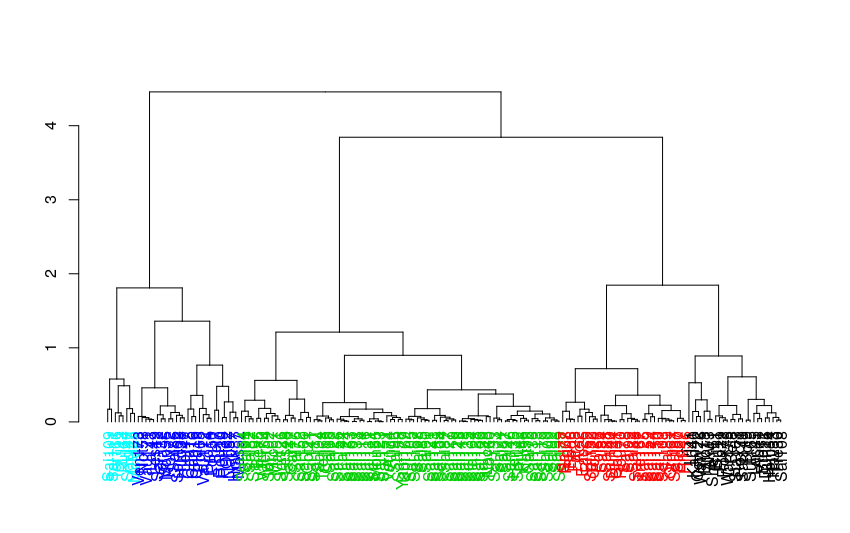
\includegraphics[width=\textwidth]{thesis/figures/clustering_values.png}
%  \caption{Results of Ward clustering for land use for municipalities (cut at 5 groups).}
%  \label{fig:clustervals}
% \end{figure}
% 
% % TRANSITIONS
% \begin{figure}[h!]
%     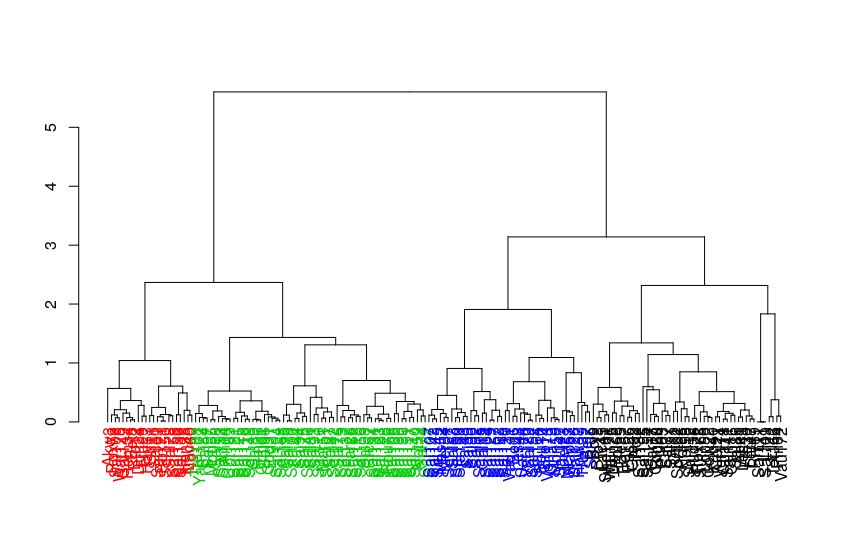
\includegraphics[width=\textwidth]{thesis/figures/clustering_trans.png}
%   \caption{Results of Ward clustering for transition data for municipalities (cut at 4 groups).}
%   \label{fig:clustertrans}
% \end{figure}

%---------------------------------------------------------------------------------------------------------------------------------------------------
% ROC Curves

% Agex

% \begin{figure}[h!]
% \makebox[\textwidth]{
%   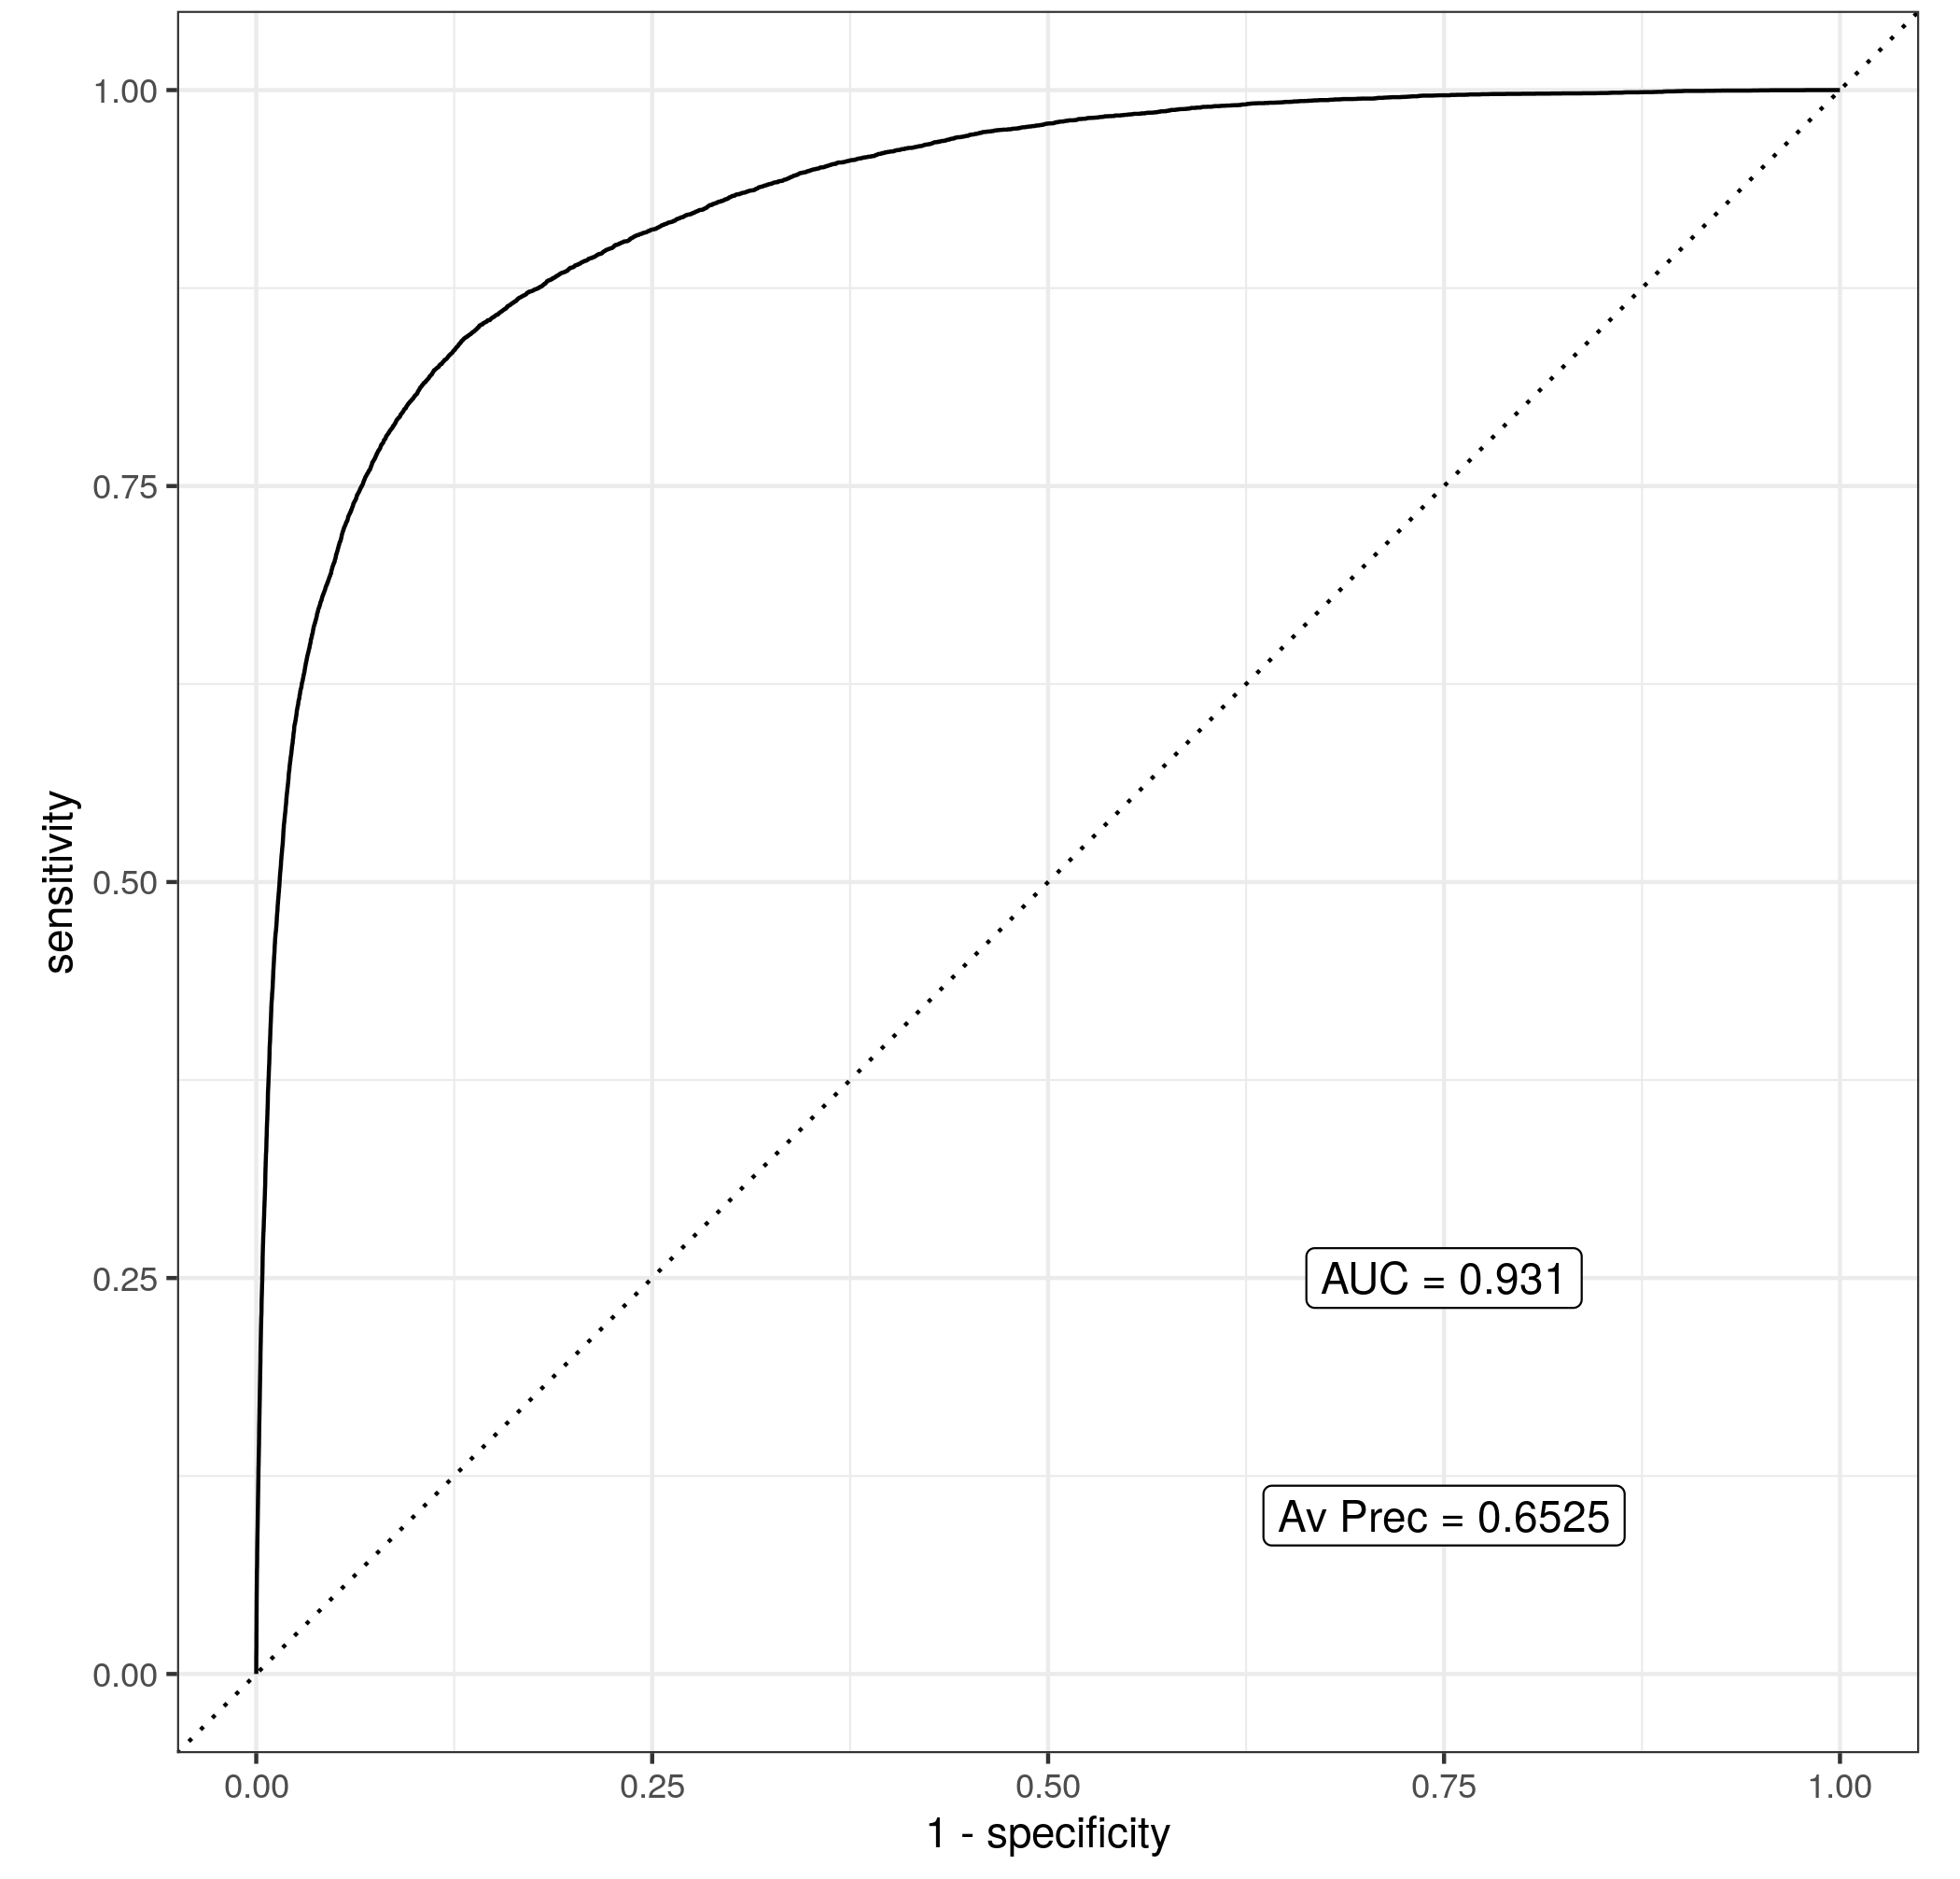
\includegraphics[width=\textwidth]{thesis/figures/rf_ratio_2_agex_roc.png}
% }
%  \caption{ROC Curve for Agricultural Expansion.}
%  \label{fig:roc_agex}
% \end{figure}
% 
% % Urb
% 
% \begin{figure}[h!]
% \makebox[\textwidth]{
%   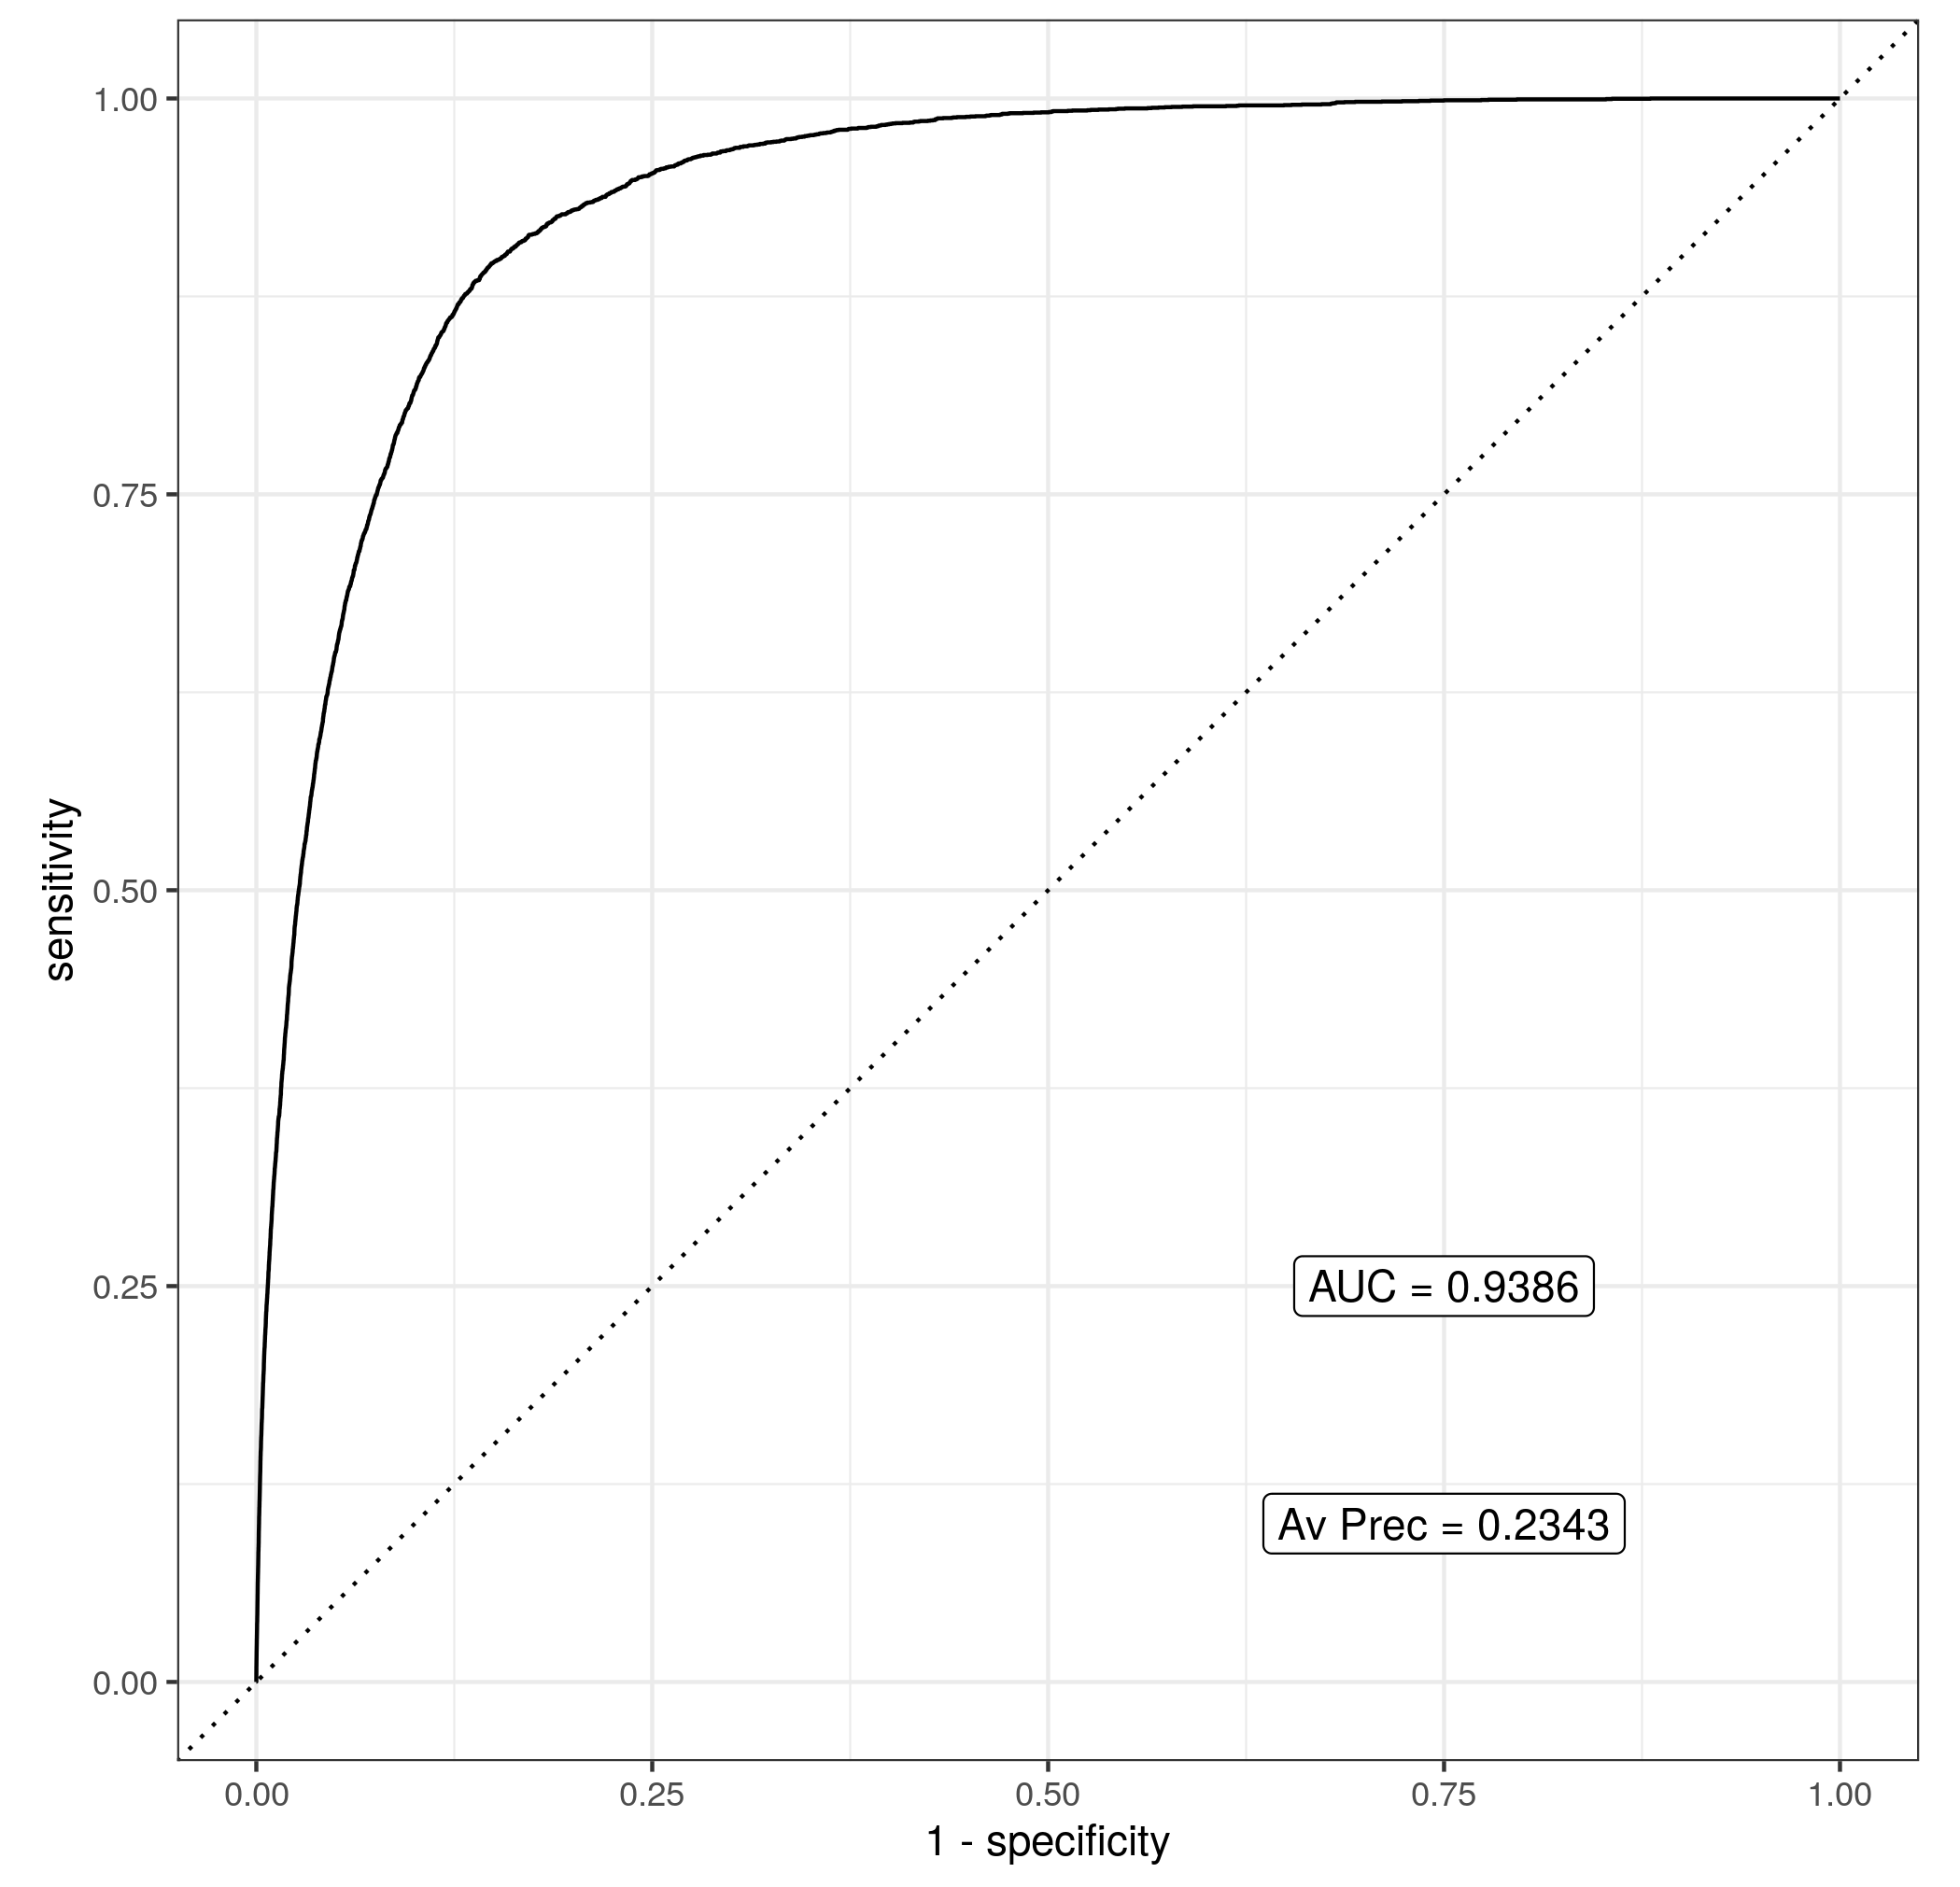
\includegraphics[width=\textwidth]{thesis/figures/rf_ratio_2_urb_roc.png}
% }
%  \caption{ROC Curve for Urbanisation.}
%  \label{fig:roc_urb}
% \end{figure}

%  Resample, figure and table

\begin{figure}[h!]
\makebox[\textwidth]{
  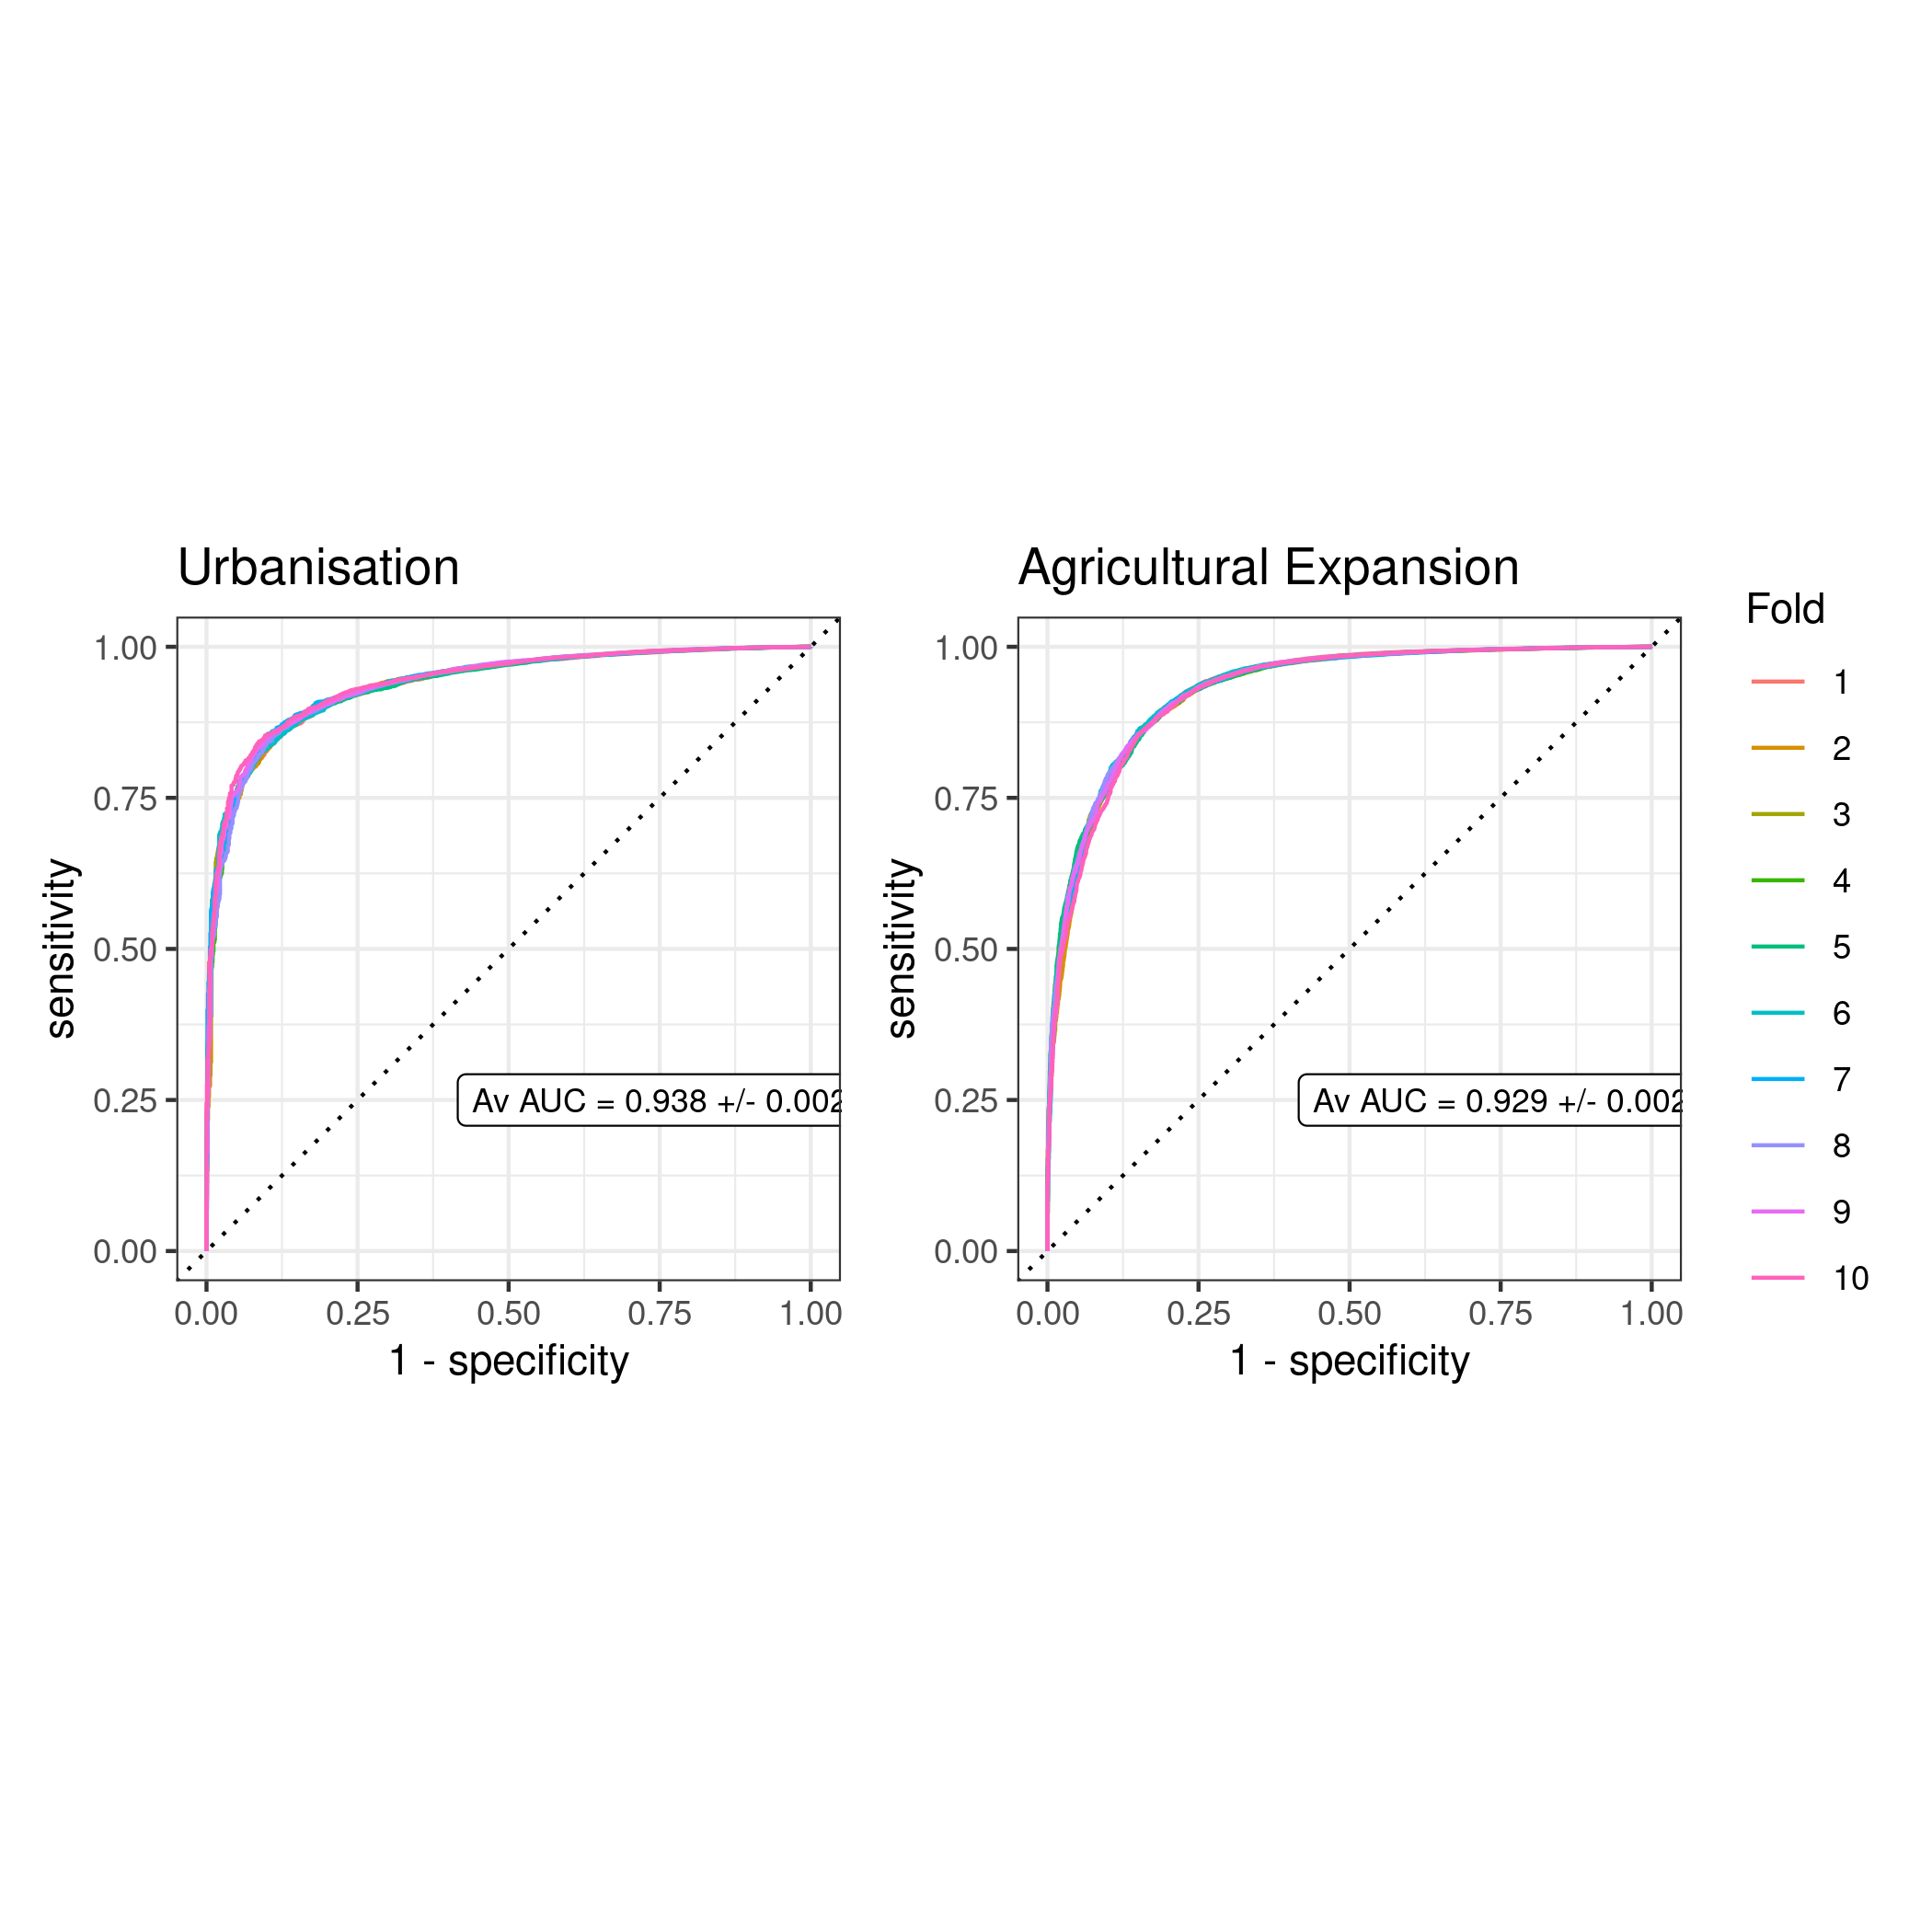
\includegraphics[width=1.3\textwidth]{thesis/figures/double_roc_resample.png}
}
 \caption{ROC Curves for re-samples for both Agricultural Expansion and Urbanisation.}
 \label{fig:roc_rs}
\end{figure}

%---------------------------------------------------------------------------------------------------------------------------------------------------
% Maps compare

\begin{figure}[h!]
\makebox[\textwidth]{
  \includegraphics[width=1.3\textwidth]{thesis/figures/scenario_39_compare.png}
}
 \caption{Comparison of Montérégie at the beginning of the BAU scenario in 2010, and at the end in 2100 (under baseline climate scenario).}
 \label{fig:BAU_compare}
\end{figure}

\begin{figure}[h!]
\makebox[\textwidth]{
  \includegraphics[width=1.3\textwidth]{thesis/figures/scenario_42_compare.png}
}
 \caption{Comparison of Montérégie at the beginning of the Reforestation scenario in 2010, and at the end in 2100 (under baseline climate scenario).}
 \label{fig:Ref_compare}
\end{figure}

\newpage

%---------------------------------------------------------------------------------------------------------------------------------------------------

\chapter*{\textbf{Chapter II Supplementary Material \\ \hspace{1em}}}
\addcontentsline{toc}{chapter}{Chapter II Supplementary Material}

%---------------------------------------------------------------------------------------------------------------------------------------------------
% METHODS/results CHAP2

% Workshop tables

\begin{table}[h!]
\centering
\caption{Summary table of the community workshop: opportunities and challenges (non spatial elements).}
\label{tab:opp_chall_ns}
\begin{tabular}{m{0.15\textwidth}lm{0.5\textwidth}l}
\hline
\textbf{Table} &
  \textbf{\begin{tabular}[c]{@{}l@{}}Atout/Contrainte \\ (Opportunity/Challenge)\end{tabular}} &
  \textbf{\begin{tabular}[c]{@{}l@{}}Contenu\\ (Content)\end{tabular}} &
  \textbf{Score} \\ \hline
\multirow{5}{*}{Centre} &
  \multirow{3}{*}{Atouts} &
  Présence d'organisme environnementaux &
  8.00 \\ \cline{3-4} 
                       &                              & Basses terres: lien prioritaire l’échelle nationale & 4.00  \\ \cline{3-4} 
                       &                              & Programme ALUS                                      & 1.00  \\ \cline{2-4} 
                       & \multirow{2}{*}{Contraintes} & CPTAQ                                               & 18.00 \\ \cline{3-4} 
                       &                              & Besoin de rentabilité des entreprises agricoles     & 5.00  \\ \hline
\multirow{3}{*}{Est}   & Atouts                       & Vocation forestiere existante                       & 8.00  \\ \cline{2-4} 
                       & \multirow{2}{*}{Contraintes} & Tenure privée des terres                            & 2.00  \\ \cline{3-4} 
                       &                              & Plusieurs territoires couverts                      & 1.00  \\ \hline
\multirow{5}{*}{Nord} &
  \multirow{2}{*}{Atouts} &
  Réglementation favorable maintien couvert bois et corridor métropolitain &
  16.20 \\ \cline{3-4} 
                       &                              & PRMHH                                               & 10.80 \\ \cline{2-4} 
                       & \multirow{3}{*}{Contraintes} & Usage agricole prédominant                          & 44.33 \\ \cline{3-4} 
                       &                              & Compréhension et participation citoyenne            & 14.40 \\ \cline{3-4} 
                       &                              & Coûts pour faire de la connectivité                 & 10.80 \\ \hline
\multirow{6}{*}{Ouest} & \multirow{2}{*}{Atouts}      & Routes cours d'eau                                  & 3.00  \\ \cline{3-4} 
                       &                              & Presence de sols pauvre                             & 3.00  \\ \cline{2-4} 
                       & \multirow{4}{*}{Contraintes} & Les réalités économiques                            & 50.00 \\ \cline{3-4} 
                       &                              & Terres privées                                      & 12.00 \\ \cline{3-4} 
                       &                              & LPTAA                                               & 7.20  \\ \cline{3-4} 
                       &                              & Le monde politique                                  & 4.00  \\ \hline
\multirow{6}{*}{Montérégie} &
  \multirow{4}{*}{Atouts} &
  Milieu agricole: potentiel de faire des corridors si un levier est trouvé &
  12.60 \\ \cline{3-4} 
                       &                              & Présence d'acteurs locaux et éducation              & 8.00  \\ \cline{3-4} 
                       &                              & PRMHH                                               & 3.00  \\ \cline{3-4} 
                       &                              & Permettre l'aménagement forestier                   & 3.00  \\ \cline{2-4} 
                       & \multirow{2}{*}{Contraintes} & Routes et autoroutes                                & 4.00  \\ \cline{3-4} 
                       &                              & Terres privées, présence prédominantes              & 3.00  \\ \hline
\end{tabular}
\end{table}

% Opportunity /challenges

\begin{table}[]
\centering
\caption{Summary table of the community workshop: opportunities and challenges (spatial elements).}
\label{tab:opp_chall_s}
\begin{tabular}{m{0.15\textwidth}lm{0.5\textwidth}l}
\hline
\textbf{Table} &
  \textbf{\begin{tabular}[c]{@{}l@{}}Atout/Contrainte \\ (Opportunity/Challenge)\end{tabular}} &
  \textbf{\begin{tabular}[c]{@{}l@{}}Contenu\\ (Content)\end{tabular}} &
  \textbf{Score} \\ \hline
\multirow{5}{*}{Centre} & Atouts                       & Leaders politiques positifs                                  & 33.33          \\ \cline{2-4} 
                        & Les deux                     & Propriétés protégées                                         & 26.67          \\ \cline{2-4} 
                        & \multirow{3}{*}{Contraintes} & Pressions urbaines                                           & 42.86          \\ \cline{3-4} 
                        &                              & Manque d'adhésion des agriculteurs                           & 39.29          \\ \cline{3-4} 
                        &                              & Pressions agricoles                                          & 16.20          \\ \hline
\multirow{5}{*}{Est}          & Atouts                       & Mobilisation projet corridor bleu vert fondation séthy                         & 18.00 \\ \cline{2-4} 
                        & \multirow{4}{*}{Contraintes} & Autoroute 10                                                 & 26.67          \\ \cline{3-4} 
                        &                              & Pressions villegiatives                                      & 22.2           \\ \cline{3-4} 
                        &                              & Fragmentation des habitats liées au dev                      & 18.00          \\ \cline{3-4} 
                        &                              & Activites agricoles intensives                               & 16.2           \\ \hline
\multirow{4}{*}{Nord}         & \multirow{2}{*}{Atouts}      & Municipalite pro-protection des monteregiennes ex. st bruno mont saint hilaire & 8.00  \\ \cline{3-4} 
                        &                              & Comité municipal travail MRC MDY                             & 1.00           \\ \cline{2-4} 
                        & \multirow{2}{*}{Contraintes} & Autoroute 10 20 30 et autres                                 & 1.00           \\ \cline{3-4} 
                        &                              & Gestion de l'application des bandes riveraines               & 1.00           \\ \hline
\multirow{6}{*}{Ouest}  & \multirow{4}{*}{Atouts}      & Proximité des milieux                                        & 24.00          \\ \cline{3-4} 
                        &                              & Article 50.3 du règlement des exploitations agricoles        & 19.20          \\ \cline{3-4} 
                        &                              & Mobilisation des acteurs du milieux                          & 12.00          \\ \cline{3-4} 
                        &                              & Bande riveraine potentielle                                  & 10.00          \\ \cline{2-4} 
                        & \multirow{2}{*}{Contraintes} & Canal beauharnois isole                                      & 24.00          \\ \cline{3-4} 
                        &                              & Réticences de certains producteurs                           & 10.00          \\ \hline
\multirow{5}{*}{Montérégie 1} & \multirow{3}{*}{Atouts}      & Réseaux de sites avec couvert forestier                                        & 14.4  \\ \cline{3-4} 
                        &                              & Grande volonté d'action locale pour créer de la connectivité & 12.60          \\ \cline{3-4} 
                        &                              & Rétrécissement du fleuve                                     & 7.20           \\ \cline{2-4} 
                              & \multirow{2}{*}{Contraintes} & Agriculture intensive compenser la production                                  & 16.20 \\ \cline{3-4} 
                        &                              & Développement urbain                                         & 12.00          \\ \hline
\multirow{5}{*}{Montérégie 2} & \multirow{2}{*}{Atouts}      & Mobilisation sociale organisme conservation sensibilisation                    & 12.00 \\ \cline{3-4} 
                        &                              & Usage des sols favorable                                     & 10.00          \\ \cline{2-4} 
                        & \multirow{3}{*}{Contraintes} & Prix des terres agricoles                                    & 12.00          \\ \cline{3-4} 
                        &                              & Étalement urbain deuxième couronne                           & 10.00          \\ \cline{3-4} 
                        &                              & Pole logistique de transport                                 & 10.00          \\ \hline
\end{tabular}
\end{table}

\begin{table}[h!]
\centering
\caption{Breakdown of the administrative districts (MRCs) covered by each table in the workshop.}
\label{tab:workshoptables}
\begin{tabular}{ll}
\hline
\textbf{Table} & \textbf{MRCs} \\ \hline
Ouest (West) & Vaudreuil, Haut SL, Beauharnois \\
Centre (Center) & Jardins, Haut Richelieu, Rouville, Roussillon \\
Nord (North) & \begin{tabular}[c]{@{}l@{}}Longueuil, Marguerite d'Youville, Vallée du richelieu, \\ Pierre de Saurel, Les Maskoutains\end{tabular} \\
Est & Brome-Missisquoi, Haute Yamaska, Acton \\
Transversal (x2) & Toute la Montérégie (All of  Montérégie)\\ \hline
\end{tabular}
\end{table}

%---------------------------------------------------------------------------------------------------------------------------------------------------
% Maps compare

\begin{figure}[h!]
\makebox[\textwidth]{
  \includegraphics[width=1.3\textwidth]{thesis/figures/scenario_45_compare.png}
}
 \caption{Comparison of Montérégie at the beginning of the Corridor protection scenario in 2010, and at the end in 2100 (under baseline climate scenario).}
 \label{fig:Corr_compare}
\end{figure}

\begin{figure}[h!]
\makebox[\textwidth]{
  \includegraphics[width=1.3\textwidth]{thesis/figures/scenario_48_compare.png}
}
 \caption{Comparison of Montérégie at the beginning of the Corridor protection + Reforestation scenario in 2010, and at the end in 2100 (under baseline climate scenario).}
 \label{fig:	CorrRef_compare}
\end{figure}

\begin{figure}[h!]
\makebox[\textwidth]{
  \includegraphics[width=1.3\textwidth]{thesis/figures/scenario_51_compare.png}
}
 \caption{Comparison of Montérégie at the beginning of the Corridor protection + Targeted Reforestation scenario in 2010, and at the end in 2100 (under baseline climate scenario).}
 \label{fig:	CorrRefT_compare}
\end{figure}

%---------------------------------------------------------------------------------------------------------------------------------------------------
% Flow

% Radar All
\begin{figure}[h!]
\makebox[\textwidth]{
  \includegraphics[width=1.3\textwidth]{thesis/figures/radar_ggradar_both.png}
}
 \caption{Change in mean flow (in \% of the 2010 flow) between 2010 (observed) and 2100 (predicted), contrasting BAU scenario (solid line) with all other scenarios from borth chapters - radar graph.}
 \label{fig:flow_radar_both}
\end{figure}